\documentclass[10pt,a4paper]{article}

\usepackage[utf8]{inputenc}
\usepackage[T1]{fontenc}
\usepackage[margin=1.85cm]{geometry}
\usepackage{amsmath}
\usepackage{array}
\usepackage{booktabs}
\usepackage{float}
\usepackage{graphicx}
\usepackage{hyperref}
\usepackage{pgfplots}
\usepackage{siunitx}
\usepackage{tikz}

\pgfplotsset{compat=1.18}
\hypersetup{
    colorlinks=true,
    linkcolor=black,
    citecolor=black,
    urlcolor=blue
}

\setlength{\parindent}{0pt}
\setlength{\parskip}{0.45em}
\renewcommand{\arraystretch}{1.08}

\title{\textbf{Learning to Play Bubble Shooter with Masked Proximal Policy Optimization}\\
\large AE4350 Bio-Inspired Intelligence Assignment}
\author{Matias Förrer\\
Student number: 4838661\\
\href{mailto:m.a.forrer@student.tudelft.nl}{m.a.forrer@student.tudelft.nl}\\
Repository: \url{https://github.com/MatiasForrer/Bubble_Bio_Game.git}}
\date{\today}

\begin{document}
\maketitle

\begin{abstract}
This report investigates whether a reinforcement learning agent can learn an effective scoring and survival strategy in a custom Bubble Shooter-style game. The project implements a Gymnasium-compatible environment with a staggered hexagonal board, stochastic bubble colours, legal-shot constraints, group popping, floating-cluster removal, board scrolling and shaped rewards. The learning method is Maskable Proximal Policy Optimization (Maskable PPO), which removes illegal actions from the policy distribution before sampling or deterministic prediction. The initial experiments use a compact \(8\times10\) board with 80 encoded actions. The project is then extended to a full-size \(13\times17\) board with 221 encoded actions, making board scale a direct scalability experiment. On 50 held-out small-board test episodes, valid-random play obtains \(480.90 \pm 105.95\) score, while the best trained policies obtain approximately 1350 score. On the full board, valid-random play obtains \(1094.70 \pm 170.97\), while the 1M-step final PPO model obtains \(1679.20 \pm 292.86\). The results show clear learning beyond random legal play, while also showing that final checkpoints, validation-best checkpoints and held-out-test-best policies do not always coincide.
\end{abstract}

\section{Introduction}

Reinforcement learning (RL) studies how an agent can improve behaviour by interacting with an environment and receiving scalar rewards. This trial-and-error formulation is closely aligned with bio-inspired intelligence: rather than specifying a complete decision rule by hand, the agent adapts a policy from experience. Sutton and Barto define RL as learning to choose actions that maximize cumulative reward under uncertainty \cite{SuttonBarto2018}. The AE4350 assignment allows computer-game tasks because they contain the essential closed loop of perception, action, environmental response and reward.

This project studies a simplified Bubble Shooter game, called \textit{Bio Bubble}. The agent observes the current bubble grid and the next bubble colour, then chooses a target cell. If this creates a connected same-colour group of at least three bubbles, the group is removed. Detached floating bubbles are removed as well. The board scrolls downward every second valid move, so the agent must both score points and prevent the board from reaching the bottom.

The research question is:
\begin{quote}
\textit{Can a PPO-based reinforcement learning agent learn a robust scoring and survival policy for a stochastic Bubble Shooter environment, and how do training budget, rollout length, checkpoint selection and board scale affect performance?}
\end{quote}

The main contributions are:
\begin{itemize}
    \item a custom Gymnasium Bubble Shooter environment with staggered hex-grid dynamics;
    \item legal-action masking that includes invalid cells, occupied cells and shot visibility;
    \item PPO training with automatic validation-based checkpoint selection;
    \item sensitivity analysis over training budget and \texttt{n\_steps};
    \item a full-board scalability experiment using a \(13\times17\) board.
\end{itemize}

\section{Environment and MDP}

\subsection{Game Dynamics}

The game is a discrete single-agent environment. A cell value of \(-1\) represents invalid padding in short shifted rows, 0 represents an empty valid cell, and values 1--3 represent bubble colours. The small board uses width 8 and height 10; the full board uses width 13 and height 17, matching the observed full game layout with 13-cell wide rows and 12-cell shifted rows.

\begin{table}[H]
\centering
\caption{The full board increases the state and action dimensions substantially, making it a useful scalability test rather than merely a cosmetic change.}
\label{tab:board-variants}
\small
\begin{tabular}{lrrrrr}
\toprule
Variant & Width & Height & Encoded actions & Start rows & Max rounds \\
\midrule
Small board & 8 & 10 & 80 & 2 & 40 \\
Full board & 13 & 17 & 221 & 5 & 80 \\
\bottomrule
\end{tabular}
\end{table}

The full board is harder for five reasons. First, the encoded action space grows from 80 to 221 actions. Second, the observation tensor grows from \(10\times8\) to \(17\times13\). Third, each action mask requires more legal-shot calculations. Fourth, episodes can last longer. Fifth, actions have more delayed consequences because there is more vertical space before a bottom-row loss. Models trained on the small board cannot be reused directly on the full board, because the policy input and output dimensions change.

\begin{figure}[H]
\centering
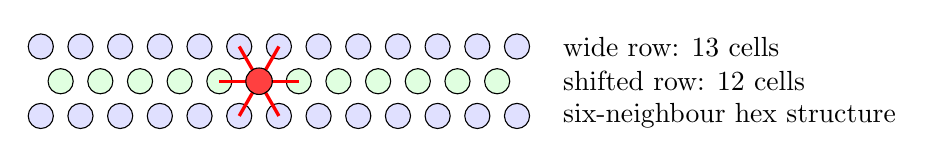
\begin{tikzpicture}[scale=0.42]
    \coordinate (selected) at (6.6,-1.05);
    \coordinate (left) at (5.4,-1.05);
    \coordinate (right) at (7.8,-1.05);
    \coordinate (upperleft) at (6.0,0);
    \coordinate (upperright) at (7.2,0);
    \coordinate (lowerleft) at (6.0,-2.1);
    \coordinate (lowerright) at (7.2,-2.1);

    \foreach \x in {0,...,12} {
        \draw[fill=blue!12] (\x*1.2,0) circle (0.38);
    }
    \foreach \x in {0,...,11} {
        \draw[fill=green!12] (\x*1.2+0.6,-1.05) circle (0.38);
    }
    \foreach \x in {0,...,12} {
        \draw[fill=blue!12] (\x*1.2,-2.1) circle (0.38);
    }

    \draw[very thick,red] (selected) -- (left);
    \draw[very thick,red] (selected) -- (right);
    \draw[very thick,red] (selected) -- (upperleft);
    \draw[very thick,red] (selected) -- (upperright);
    \draw[very thick,red] (selected) -- (lowerleft);
    \draw[very thick,red] (selected) -- (lowerright);

    \draw[fill=red!75] (selected) circle (0.4);

    \node[anchor=west] at (15.5,0) {wide row: 13 cells};
    \node[anchor=west] at (15.5,-1.05) {shifted row: 12 cells};
    \node[anchor=west] at (15.5,-2.1) {six-neighbour hex structure};
\end{tikzpicture}
\caption{Staggered hex layout used by the full board. The red edges show the six-neighbour relation around one cell.}
\label{fig:hex-grid}
\end{figure}

\subsection{MDP Formulation}

The environment can be written as a finite Markov decision process
\[
\mathcal{M}=(\mathcal{S},\mathcal{A},P,R,\gamma).
\]
The state \(s_t\in\mathcal{S}\) contains the board grid, the next bubble colour and the stagger offset. The action \(a_t\in\mathcal{A}\) is an encoded target cell \(a_t=yW+x\). The transition distribution \(P(s_{t+1}\mid s_t,a_t)\) is stochastic because new rows and next bubble colours are sampled randomly. The reward \(R(s_t,a_t,s_{t+1})\) is the shaped RL reward described below. The discount factor \(\gamma\) is handled by PPO internally. Episodes terminate when a bottom-row bubble appears, no legal actions remain, or the maximum round count is reached.

\begin{table}[H]
\centering
\caption{Notation used throughout the report.}
\label{tab:notation}
\small
\begin{tabular}{ll}
\toprule
Symbol & Meaning \\
\midrule
\(s_t\) & Environment state at time \(t\): grid, next colour and stagger offset \\
\(a_t\) & Encoded target-cell action at time \(t\) \\
\(R_t\) & Scalar reward given to the learning algorithm \\
\(N_{\mathrm{pop}}\) & Number of directly popped same-colour bubbles \\
\(N_{\mathrm{float}}\) & Number of detached floating bubbles removed \\
\(m(s,a)\) & Binary legal-action mask for action \(a\) in state \(s\) \\
\bottomrule
\end{tabular}
\end{table}

\subsection{Action Masking}

The encoded action space contains many illegal actions. A cell may be outside a shifted row, already occupied, disconnected from the ceiling or existing bubbles, or unreachable due to blocked shot paths. The legal-action mask is
\[
m(s,a)\in\{0,1\},
\]
where \(m(s,a)=1\) means action \(a\) is legal in state \(s\). Maskable PPO applies this mask before sampling or prediction:
\[
\pi_{\mathrm{masked}}(a\mid s)=
\frac{\pi(a\mid s)m(s,a)}
{\sum_{a'\in\mathcal{A}}\pi(a'\mid s)m(s,a')}.
\]
This prevents the policy from wasting probability mass on impossible actions. Invalid action masking is especially relevant in large discrete action spaces where only a subset of actions is valid at each state \cite{HuangOntanon2020}.

\subsection{Reward and Score}

The human score is used for reporting performance. The RL reward is used for training and follows the same qualitative incentives: pop bubbles, remove floating clusters, make large clears, survive, and avoid game over.
\[
R_t =
-1
+2N_{\mathrm{pop}}
+3N_{\mathrm{float}}
+B(N_{\mathrm{pop}}+N_{\mathrm{float}})
+1.5I_{\mathrm{survive}}
-25I_{\mathrm{gameover}},
\]
where \(B(n)=6\) if \(n\geq8\), \(B(n)=2.5\) if \(5\leq n<8\), and \(B(n)=0\) otherwise.

\begin{table}[H]
\centering
\caption{Reward shaping gives the agent intermediate feedback for useful sub-goals, while the reported game score remains interpretable to a human player.}
\label{tab:reward}
\small
\begin{tabular}{lll}
\toprule
Event & Human score & RL reward \\
\midrule
Turn cost & 0 & \(-1.0\) \\
Directly popped bubble & \(+10\) each & \(+2.0\) each \\
Floating bubble removed & \(+15\) each & \(+3.0\) each \\
Clear at least 5 bubbles & \(+25\) & \(+2.5\) \\
Clear at least 8 bubbles & \(+60\) & \(+6.0\) \\
Survive move & \(+5\) & \(+1.5\) \\
Game over & 0 directly & \(-25.0\) \\
\bottomrule
\end{tabular}
\end{table}

\section{Learning Method}

\subsection{PPO and Hyperparameters}

The agent is trained with Proximal Policy Optimization (PPO), a policy-gradient method that improves a stochastic policy while limiting destructive policy updates through a clipped surrogate objective \cite{Schulman2017}. Stable-Baselines3 provides the PPO implementation and SB3-Contrib provides Maskable PPO \cite{SB3PPO,SB3MaskablePPO}. The policy type is \texttt{MultiInputPolicy}, because the observation is a dictionary.

\begin{table}[H]
\centering
\caption{Training hyperparameters and their roles. These are reported to make the experiment reproducible.}
\label{tab:hyperparameter-definitions}
\small
\begin{tabular}{lll}
\toprule
Hyperparameter & Main value & Definition \\
\midrule
\texttt{n\_steps} & 512 or 128 & Rollout length collected before each PPO update \\
\texttt{batch\_size} & 128 & Minibatch size during gradient optimization \\
\texttt{n\_epochs} & 10 & Optimization passes over each rollout buffer \\
Learning rate & \(3\times10^{-4}\) & Step size for policy and value-network updates \\
Evaluation mode & deterministic & Uses the most likely legal action for testing \\
Validation interval & 25,000 & Timesteps between checkpoint evaluations \\
Validation episodes & 10 & Fixed-seed episodes for model selection \\
\bottomrule
\end{tabular}
\end{table}

\subsection{Training Procedure}

\begin{figure}[H]
\centering
\fbox{
\begin{minipage}{0.92\linewidth}
\small
\textbf{Masked PPO training loop}\\
1. Reset \texttt{BubblePopEnv} and observe grid, next bubble and stagger offset.\\
2. Compute the legal-action mask \(m(s_t,a)\).\\
3. Maskable PPO samples a legal action from \(\pi_{\mathrm{masked}}(a_t\mid s_t)\).\\
4. The environment applies the shot to the selected board cell.\\
5. Same-colour groups pop; floating clusters are removed; the board may scroll.\\
6. PPO updates the policy after \texttt{n\_steps} collected transitions.\\
7. Every 25k timesteps, evaluate deterministically on fixed validation seeds and save a new best checkpoint if average score improves.
\end{minipage}}
\caption{Training pipeline used by the implemented scripts. The same action mask is used during training, validation and watching.}
\label{fig:pseudocode}
\end{figure}

Models are saved with filenames that record date, time, timesteps, rollout length and environment dimensions. For example:
\begin{verbatim}
bubble_pop_model_20260827_210357_ts500000_nsteps512_w13_h17_c3_
start5_rounds80_move2_best_step375000_avg1840.zip
\end{verbatim}
This naming convention makes it possible to select the correct environment when watching a trained model.

\section{Experimental Setup}

\subsection{Configurations}

\begin{table}[H]
\centering
\caption{Main experiments. All learned agents use Maskable PPO unless stated otherwise.}
\label{tab:configs}
\small
\begin{tabular}{lrrrrrr}
\toprule
Experiment & Width & Height & Timesteps & \texttt{n\_steps} & Start rows & Max rounds \\
\midrule
Small-board budget tests & 8 & 10 & 250k--1M & 512 & 2 & 40 \\
Small-board rollout test & 8 & 10 & 500k & 128 & 2 & 40 \\
Full-board scale test & 13 & 17 & 500k & 512 & 5 & 80 \\
Full-board extended test & 13 & 17 & 1M & 512 & 5 & 80 \\
\bottomrule
\end{tabular}
\end{table}

The held-out evaluation uses seeds 2000--2049. These are independent of the validation seeds 1000--1009 used for checkpoint selection. For each policy, 50 deterministic episodes are evaluated. The random baseline is a valid-random baseline: it samples uniformly from the legal action mask, so it is stronger than a naive random policy that attempts illegal moves.

The 95\% confidence interval is
\[
\bar{x}\pm1.96\frac{s}{\sqrt{n}},
\]
where \(\bar{x}\) is the sample mean, \(s\) is the sample standard deviation and \(n=50\).

\section{Results}

\subsection{Small-Board Performance}

\begin{table}[H]
\centering
\caption{Held-out small-board results show that PPO consistently outperforms valid-random play, while overlapping confidence intervals mean the top policies should not be over-ranked.}
\label{tab:small-results}
\small
\begin{tabular}{lrrrrrrr}
\toprule
Policy & Mean & CI95 & Median & Std. & Max & Rounds & Wins \\
\midrule
Valid random & 480.90 & 105.95 & 392.50 & 382.22 & 1460 & 15.10 & -- \\
500k, \texttt{n\_steps}=512, best & 1083.70 & 160.44 & 972.50 & 578.80 & 2725 & 21.98 & 43 \\
500k, \texttt{n\_steps}=128, best & 1216.90 & 214.86 & 1015.00 & 775.16 & 3110 & 24.04 & 41 \\
500k, \texttt{n\_steps}=128, final & \textbf{1354.50} & 237.73 & \textbf{1207.50} & 857.67 & \textbf{3060} & \textbf{25.86} & 38 \\
1M, \texttt{n\_steps}=512, best & 1353.10 & 215.82 & 1140.00 & 778.63 & 2905 & 25.40 & \textbf{45} \\
\bottomrule
\end{tabular}
\end{table}

All trained policies obtain substantially higher scores and survive longer than valid-random play. The best average scores are around 1350, almost three times the random baseline mean. The 1M best checkpoint has the highest number of matched-seed wins against random, while the 500k \(\texttt{n\_steps}=128\) final model has the highest held-out mean. Because confidence intervals overlap, the robust conclusion is that both are strong learned policies, not that one is conclusively superior.

\subsection{Full-Board Performance}

\begin{table}[H]
\centering
\caption{The full-board experiment confirms scalability to a 221-action environment, but the relative improvement over valid-random play is smaller than on the compact board.}
\label{tab:full-results}
\small
\begin{tabular}{lrrrrrr}
\toprule
Policy & Mean & CI95 & Median & Max & Rounds & Wins \\
\midrule
Full-board valid random & 1094.70 & 170.97 & 995.00 & 2605 & 23.46 & -- \\
Full-board 500k final & 1488.50 & 170.70 & \textbf{1372.50} & 3300 & 26.16 & \textbf{37} \\
Full-board 500k best & 1469.40 & 206.13 & 1282.50 & \textbf{4370} & 26.12 & 33 \\
Full-board 1M final & \textbf{1679.20} & 292.86 & 1347.50 & \textbf{4940} & \textbf{28.00} & \textbf{37} \\
Full-board 1M best & 1495.00 & 239.15 & 1317.50 & 4695 & 26.30 & 34 \\
\bottomrule
\end{tabular}
\end{table}

The full-board random baseline is stronger in absolute score because the board is larger, starts with more bubbles and permits longer games. PPO improves the average score by about 375--394 points after 500k timesteps and by 584.50 points after 1M timesteps. The 1M final model is the strongest full-board model on held-out mean score, while the 1M validation-best checkpoint is weaker on held-out testing. This again shows that validation-selected and test-best policies need not be identical.

\subsection{Validation and Test Plots}

\begin{figure}[H]
\centering
\begin{minipage}{0.49\linewidth}
\centering
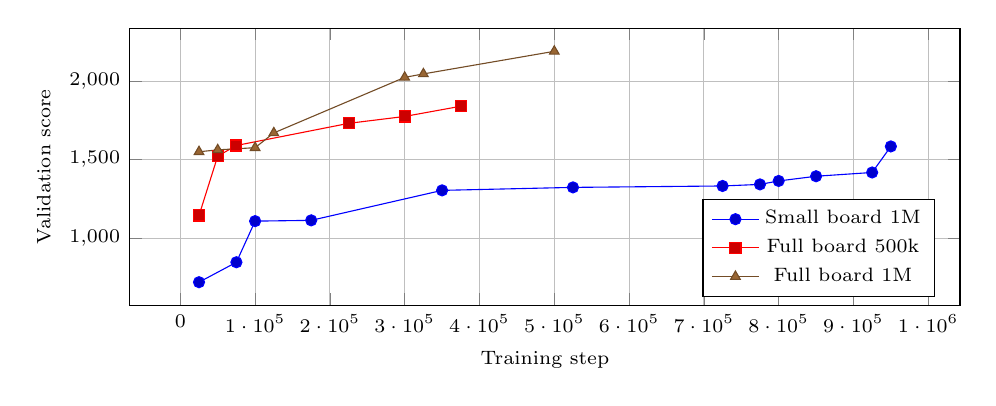
\begin{tikzpicture}
\begin{axis}[
    width=\linewidth,
    height=5.1cm,
    xlabel={Training step},
    ylabel={Validation score},
    legend pos=south east,
    grid=major,
    scaled x ticks=false,
    tick label style={font=\scriptsize},
    label style={font=\scriptsize},
    legend style={font=\scriptsize}
]
\addplot+[mark=*] coordinates {
    (25000,719) (75000,846) (100000,1108) (175000,1113)
    (350000,1304) (525000,1323) (725000,1332)
    (775000,1342) (800000,1364) (850000,1394)
    (925000,1418) (950000,1584)
};
\addlegendentry{Small board 1M}
\addplot+[mark=square*] coordinates {
    (25000,1144) (50000,1522) (75000,1590)
    (225000,1731) (300000,1775) (375000,1840)
};
\addlegendentry{Full board 500k}
\addplot+[mark=triangle*] coordinates {
    (25000,1550) (50000,1562) (100000,1576)
    (125000,1670) (300000,2024) (325000,2046)
    (500000,2190)
};
\addlegendentry{Full board 1M}
\end{axis}
\end{tikzpicture}
\end{minipage}
\begin{minipage}{0.49\linewidth}
\centering
\begin{tikzpicture}
\begin{axis}[
    width=\linewidth,
    height=5.1cm,
    ybar,
    bar width=5pt,
    ylabel={Held-out mean score},
    symbolic x coords={Rand,500k-512,500k-128,1M-512,FullRand,Full500k,Full1MFinal,Full1MBest},
    xtick=data,
    x tick label style={rotate=35,anchor=east,font=\scriptsize},
    tick label style={font=\scriptsize},
    label style={font=\scriptsize},
    ymin=0,
    grid=major,
    error bars/.cd,
    y dir=both,
    y explicit
]
\addplot+[error bars/.cd, y explicit] coordinates {
    (Rand,480.90) +- (0,105.95)
    (500k-512,1083.70) +- (0,160.44)
    (500k-128,1354.50) +- (0,237.73)
    (1M-512,1353.10) +- (0,215.82)
    (FullRand,1094.70) +- (0,170.97)
    (Full500k,1488.50) +- (0,170.70)
    (Full1MFinal,1679.20) +- (0,292.86)
    (Full1MBest,1495.00) +- (0,239.15)
};
\end{axis}
\end{tikzpicture}
\end{minipage}
\caption{Validation curves show checkpoint improvement during training. Held-out score bars show that learned policies outperform valid-random baselines, but top-policy uncertainty intervals overlap.}
\label{fig:results-plots}
\end{figure}

\section{Sensitivity Analysis}

\subsection{Training Budget}

Training budget strongly affects whether a useful policy is found. On the small board, 250k timesteps already produced a policy far above random in earlier evaluation, and the 1M run produced the strongest validation checkpoint. The validation curve in Figure~\ref{fig:results-plots} continues improving late in the small-board 1M run, reaching its best checkpoint at 950k timesteps. On the full board, the 1M run reached a validation average of 2190 and improved the held-out mean from 1488.50 for the 500k final model to 1679.20 for the 1M final model. This indicates that the larger board benefited from additional training.

\subsection{Rollout Length}

The comparison between \(\texttt{n\_steps}=512\) and \(\texttt{n\_steps}=128\) is a real hyperparameter sensitivity result. Reducing rollout length did not harm performance: the 500k \(\texttt{n\_steps}=128\) final policy achieved a held-out mean of 1354.50, compared with 1083.70 for the 500k \(\texttt{n\_steps}=512\) best checkpoint in the same table. This suggests that more frequent policy updates may help in this discrete game. The caveat is that run-to-run variance is large, so this should be interpreted as evidence of sensitivity, not a definitive proof that 128 is always better.

\subsection{Checkpoint Selection}

Checkpoint selection matters because the final model is not always the best model under either validation or held-out testing. In the small-board 1M run, the validation-best checkpoint is stronger than the final checkpoint in previous fixed-seed checks. In the full-board 500k and 1M runs, however, the final models outperformed the validation-best checkpoints on held-out mean score. This difference is scientifically useful: validation selection helps avoid bad final policies, but final conclusions must use independent test seeds.

\subsection{Board Scale}

Scaling from \(8\times10\) to \(13\times17\) changes the problem qualitatively. The small board shows a large relative improvement over random play. The full board still improves over random, but the margin is smaller: after 1M timesteps the final full-board model improves by 584.50 mean score points over valid-random play. This is consistent with the larger action space, larger observation space and longer-horizon consequences. The full-board experiment therefore strengthens the report's environment-complexity score while showing that larger games require more training to obtain clear gains.

\section{Analysis of the Learned Solution}

To inspect the policy, deterministic actions from the trained small-board 1M best checkpoint were recorded. Table~\ref{tab:policy-examples} shows three representative decisions. The board fragments are the upper rows before the selected action; dots are empty cells.

\begin{table}[H]
\centering
\caption{Actual policy examples show that the trained agent often chooses placements that create immediate clears or floating removals, but can still fail in crowded states.}
\label{tab:policy-examples}
\scriptsize
\begin{tabular}{p{0.16\linewidth}p{0.46\linewidth}p{0.30\linewidth}}
\toprule
Case & Board before action & Action and result \\
\midrule
Large clear, seed 2000 &
\texttt{r0: 2 3 1 1 1 1 2 3}\newline
\texttt{r1: \ \ 2 2 2 1 2 3 3}\newline
\texttt{r2: 1 2 1 2 1 1 2 2}\newline
\texttt{r3: \ \ . . 1 . 2 . .}
&
Next colour 1, action \((3,3)\). Result: \(N_{\mathrm{pop}}=10\), \(N_{\mathrm{float}}=1\), score \(+180\). \\
\midrule
Medium clear, seed 2001 &
\texttt{r0: 1 3 2 1 3 2 2 2}\newline
\texttt{r1: \ \ 1 2 1 2 3 3 1}\newline
\texttt{r2: 1 2 1 1 2 2 1 3}\newline
\texttt{r3: \ \ . . 2 . 3 . .}
&
Next colour 1, action \((3,3)\). Result: \(N_{\mathrm{pop}}=5\), \(N_{\mathrm{float}}=1\), score \(+95\). \\
\midrule
Failure mode, seed 2027 &
\texttt{r5: \ \ 3 2 3 3 2 1 .}\newline
\texttt{r6: 2 1 1 2 1 3 1 .}\newline
\texttt{r7: \ \ . . 2 3 . 3 .}\newline
\texttt{r8: . . 3 . . . . .}
&
Late crowded state. Action \((4,7)\) with next colour 1 produced no pop and only \(+5\) survival score. The episode ended after 13 rounds with score 205. \\
\bottomrule
\end{tabular}
\end{table}

The learned behaviour is mainly local but useful. The agent tends to attach bubbles to same-colour groups, creates immediate clears, sometimes triggers floating-cluster removals, and survives longer than random play. It also avoids many legal but unproductive low placements. The failure case shows the limitation: in crowded boards, a locally legal move can still leave the board in a poor long-term state. This is expected because the agent observes only the current board and next colour, not a sequence of future colours.

Small-board and full-board behaviour differ in scale. On the small board, the reward signal is clearer because mistakes reach the bottom quickly and good clears have immediate visible effect. On the full board, the random baseline is stronger and variance is higher because there is more room to survive and more possible placements. This explains why full-board learning is positive but less decisive after 500k timesteps.

\section{Reproducibility and Validity}

\begin{table}[H]
\centering
\caption{Software and repository information recorded for reproducibility.}
\label{tab:software}
\small
\begin{tabular}{ll}
\toprule
Item & Value \\
\midrule
Python & 3.13.14 \\
Gymnasium & 1.2.3 \\
Stable-Baselines3 & 2.8.0 \\
SB3-Contrib & 2.8.0 \\
NumPy & 2.4.3 \\
Repository remote & \url{https://github.com/MatiasForrer/Bubble_Bio_Game.git} \\
Original results branch & \texttt{backup-current-results-20260827} \\
Full-board code/results branch & \texttt{full-board-experiment-20260827} \\
\bottomrule
\end{tabular}
\end{table}

The implementation was checked with smoke tests for staggered row offsets, alternating row widths, same-colour group popping, floating-ball removal, invalid-action rejection, board-shape stability, board scrolling, game-over detection and shooter visibility.

Threats to validity remain. Training is stochastic, and only a limited number of long training runs were performed. Validation seeds are reused for checkpoint selection, so validation scores can overestimate performance. Held-out testing uses 50 episodes, which is enough to reveal clear learning but still leaves wide confidence intervals. Finally, the shaped reward may bias the learned strategy toward immediate clears rather than deeper long-horizon planning.

\section{Conclusion}

This project implemented and analysed a reinforcement learning agent for a custom Bubble Shooter environment. Maskable PPO learned policies that substantially outperform valid-random play on both the compact \(8\times10\) board and the full \(13\times17\) board. The strongest small-board policies nearly triple the random baseline mean score and survive roughly ten more rounds. The full-board experiment confirms that the method scales to a larger 221-action task, although with a smaller relative improvement.

The most important scientific finding is that learning is clear, but exact policy ranking is noisy. Training budget, rollout length and checkpoint selection all matter. The \(\texttt{n\_steps}=128\) sensitivity run performed at least as well as the \(\texttt{n\_steps}=512\) runs on held-out mean score, suggesting that frequent policy updates can be beneficial. However, overlapping confidence intervals mean that top-model rankings should be stated cautiously. Overall, the implementation and experiments satisfy the central objective: demonstrating a reproducible bio-inspired learning method that discovers effective game-playing behaviour through reward-guided interaction.

\begin{thebibliography}{9}

\bibitem{SuttonBarto2018}
R. S. Sutton and A. G. Barto.
\newblock \textit{Reinforcement Learning: An Introduction}, second edition.
\newblock MIT Press, 2018.
\newblock \url{https://mitpress.mit.edu/9780262039246/reinforcement-learning/}

\bibitem{Schulman2017}
J. Schulman, F. Wolski, P. Dhariwal, A. Radford, and O. Klimov.
\newblock Proximal Policy Optimization Algorithms.
\newblock arXiv:1707.06347, 2017.
\newblock \url{https://doi.org/10.48550/arXiv.1707.06347}

\bibitem{HuangOntanon2020}
S. Huang and S. Ontanon.
\newblock A Closer Look at Invalid Action Masking in Policy Gradient Algorithms.
\newblock arXiv:2006.14171, 2020.
\newblock \url{https://arxiv.org/abs/2006.14171}

\bibitem{GymnasiumEnv}
Farama Foundation.
\newblock Gymnasium Env API documentation.
\newblock \url{https://gymnasium.farama.org/api/env/}

\bibitem{SB3PPO}
Stable-Baselines3.
\newblock PPO documentation.
\newblock \url{https://stable-baselines3.readthedocs.io/en/v2.5.0/modules/ppo.html}

\bibitem{SB3MaskablePPO}
Stable-Baselines3 Contrib.
\newblock Maskable PPO documentation.
\newblock \url{https://sb3-contrib.readthedocs.io/en/master/modules/ppo_mask.html}

\bibitem{AE4350Assignment}
TU Delft AE4350 course team.
\newblock AE4350 Assignment Description 2025.
\newblock Local assignment PDF supplied with the project.

\end{thebibliography}

\end{document}
